% -*- mode: LaTex; outline-regexp: "\\\\section\\|\\\\subsection";fill-column: 80; -*-
\documentclass[12pt]{article}
\usepackage[longnamesfirst]{natbib}
\usepackage[usenames]{color}
\usepackage{graphicx}  % Macintosh pdf files for figures
\usepackage{bbm}       % one symbol
\usepackage{amssymb}   % Real number symbol {\Bbb R}
\input{../../standard}

% --- margins
\usepackage{../../sty/simplemargins}
\setleftmargin{1in}   % 1 inch is NSF legal minimum
\setrightmargin{1in}  % 1 inch is NSF legal minimum
\settopmargin{1in}    % 1 inch is NSF legal minimum
\setbottommargin{1in} % 1 inch is NSF legal minimum

% --- Paragraph split, indents
\setlength{\parskip}{0.00in}
\setlength{\parindent}{0in}

% --- Line spacing
\renewcommand{\baselinestretch}{1.3}

% --- Margins
\setlength{\topmargin}{-0.5in}
\setlength{\oddsidemargin}{-0.1in}
\setlength{\textheight}{9.0in}
\setlength{\textwidth}{6.5in}

% --- page numbers
\pagestyle{empty}  % so no page numbers

% --- Hypthenation
\sloppy  % fewer hyphenated
\hyphenation{stan-dard}
\hyphenation{among}

% --- Customized commands, abbreviations
\newcommand{\TIT}{{\it  {\tiny Risk inflation of alpha-investing (\today)}}}

% --- Header
\pagestyle{myheadings}
\markright{\TIT}

% --- Title

\title{ Risk Inflation of Sequential Testing }
\author{
        Dean P. Foster and Robert A. Stine\thanks{Research supported by NSF grant DMS-1106743 }  \\
        Department of Statistics            \\
        The Wharton School of the University of Pennsylvania \\
        Philadelphia, PA 19104-6340                          \\
        www-stat.wharton.upenn.edu/$\sim$stine 
}

\date{\today}


%%%%%%%%%%%%%%%%%%%%%%%%%%%%%%%%%%%%%%%%%%%%%%%%%%%%%%%%%%%%%%%%%%%%%%%%%%%

\begin{document}
\maketitle 
%------------------------------------------------------------------------

\abstract{ 

 Alpha-investing tests a possibly infinite sequence of hypotheses while
 controlling the expected number of false rejections.  This paper finds the risk
 of an estimator produced by these tests.  We characterize the worst-case risk
 of this estimator vis-a-vis an oracle.  Our analysis provides the exact risk
 inflation of alpha-investing in a finite sequence of tests.  Our results show
 that the asymptotic bound $2 \log p$ from \citet{fostergeorge94} holds for the
 alpha-investing estimator.  The best results relative to the oracle occur when
 the underlying tests are allowed to produce a surprisingly large number of
 false rejections.  Our results also characterize the population models that
 produce the maximum risk.  For example, for one type of alpha-investing, the
 model that produces the largest risk inflation has oracle risk $\log p$.

}

%------------------------------------------------------------------------
\vspace{0.05in}

\noindent
{\it Key Phrases: bellman equations, hard thresholding, testimator, variable selection}

\clearpage


% ----------------------------------------------------------------------
\section{ Introduction }
% ----------------------------------------------------------------------

 Alpha-investing is a sequential approach to multiple testing.  Rather than test
 multiple hypotheses at once, alpha-investing tests hypotheses one-at-a-time in
 a specified order.  Alpha-investing begins with an initial allowance for Type I
 error that is called its alpha-wealth.  Each test consumes some of the
 available alpha-wealth.  Alpha-investing overcomes the conservatism of
 alpha-spending procedures such as the Bonferroni method by earning a
 contribution to its alpha-wealth for each rejected null hypothesis.  Thus
 rejections beget more rejections.  Alpha-investing further allows one to test
 an infinite stream of hypotheses, accommodate dependent tests, and incorporate
 domain knowledge, all the while controlling the expected number of false
 rejections. The following section describes alpha-investing in more detail and
 provides several examples.

 
 A natural use for alpha-investing is to control of fast, sequential methods for
 building models by selecting features from a large collection of potential
 explanatory variables.  Streaming feature selection, for example, identifies
 predictive features by testing candidate predictors one-at-a-time in an order
 specified by an exogenous source rather than choosing the best from a
 predetermined collection.  Unlike stepwise regression, streaming selection
 evaluates each predictor in the context of the current model, without requiring
 knowledge of all of the other predictors that might follow.  This approach
 allows the algorithm to explore essentially infinite collections of
 explanatory variables more rapidly than possible through conventional methods
 \citep{fosterlin10, langford11}.  Because alpha-investing can test an infinite
 sequence of hypotheses, it is well-matched to a search of an unbounded
 collection of features that is too large to manipulate at once.


 Though risk or squared error may be more relevant for model selection, multiple
 testing procedures such as alpha-investing or FDR are usually evaluated from
 the perspective of controlling the rate of Type I errors.  Consider testing the
 sequence of two-sided hypotheses $H_j: \mu_j = 0$, $j = 1,\ldots, p,$ using a
 corresponding sequence of independent test statistics $Y_j \sim N(\mu_j,
 \sigma^2)$ with known variance $\sigma^2$.  The vectors $\mu = (\mu_1, \ldots,
 \mu_p)'$ and $Y = (Y_1, \ldots, Y_p)'$ collect these items.  Let the indicators
 $\gamma_j = I_{\{\beta_j\ne 0\}}$ identify the hypotheses for which $\mu_j \ne
 0$; $\gamma_j = 1$ implies $H_j$ is false.  Corresponding to these, let
 $\hat\gamma_j$ indicate which hypotheses are rejected by tests based on $Y$.
  We assume that a test rejects $H_j$ if the observed test statistic exceeds a
 threshold determined by a multiple $\hat\tau_j$ of the noise level,
 \begin{equation}
    \hat\gamma_j = I_{\{\hat\tau_j^2 \sigma^2 < Y_j^2\}} \;.  
 \label{eq:gammahat}
 \end{equation}
  $\hat\gamma_j = 1$ implies that the test rejects $H_j$ and is zero otherwise.
  Alpha-investing allows the outcome of prior tests to influence the choice of
 the threshold, so that
 \begin{equation}
   \hat\tau_j = \tau(\hat\gamma_1, \ldots, \hat\gamma_{j-1}) \;.   
 \label{eq:tauhat}
 \end{equation}
 Collect these indicators into the vectors $\gamma$ and $\hat\gamma$.  Note that
 our notation suppresses the fact that $\gamma$ is a function $\gamma(\mu)$ of
 the underlying parameters.  Let $W(\hat\gamma) = \sum_j \hat\gamma_j$ denote
 the total number of rejections, and let $V(\hat\gamma, \gamma) = \sum_j
 \hat\gamma_j (1-\gamma_j)$ count the number of false rejections.  A selector
 $\hat\gamma$ controls the expected false discovery rate (mFDR) if
 \begin{equation}
     \ev V(\hat\gamma, \gamma) \le \alpha(1 + \ev W(\hat\gamma)) \;.
 \label{eq:mfdr}
 \end{equation}
 \citet{fosterstine08} show that alpha-investing provides a generic recipe for
 constructing selectors that satisfy \eqn{eq:mfdr}.  Control of the number of
 false rejections, however, does not address the risk of the estimator.  

 
 Our objective here is to understand how well alpha-investing controls the risk
 of an estimator produced by the associated tests.  In particular, we consider
 the risk of a so-called ``testimator'' (also known as a keep-or-kill estimator
 or a hard thresholding estimator).  Given the selector $\hat\gamma$, the
 testimator $\hat\mu_{\hat\gamma} \in \Rp$ zeros out coordinates in which the
 data fail to reject $H_j$:
 \begin{equation}
   (\hat\mu_{\hat\gamma})_j 
          = \hat\mu(Y_j, \hat\tau_j) 
          = \left\{ \begin{array}{cc}
                                Y_j & \mbox{ if } \hat\tau_j^2 \sigma^2 < Y_j^2,  \cr
                                 0  & \mbox{ otherwise. }
                              \end{array}\right.
 \label{eq:muhat}
 \end{equation}
 The risk of $\hat\mu_{\hat\gamma}$ is
 \begin{equation}
    R(\hat\mu_{\hat\gamma}, \mu) 
      = \ev_\mu \normsq{\hat\mu_{\hat\gamma} - \mu} \;,
 \label{eq:risk}
 \end{equation}
 where $\normsq{x} = x'x$ for vectors $x$. 


 The risk of estimators used in orthogonal regression provide conjectures for
 the risk of estimators produced by alpha-investing.  These results do not apply
 directly because they hold for multivariate estimates produced simultaneously
 rather than sequentially.  This change in the timing of when infomatino becomes
 available affects both the estimators and the relevant oracle.  The analysis of
 risk inflation in \citet{fostergeorge94} bounds the risk of the multivariate
 estimator $\hat\mu_{\gamma(\tau)}$; this estimator uses a selector
 $\gamma(\tau)$ with a fixed threshold that rejects those $H_j$ for which
 $\tau^2 \sigma^2 < Y_j^2$.  The key difference from $\hat\mu_{\hat\gamma}$ is
 that the threshold $\tau$ is set without reference to data, being determined
 only by $p$.  \citet{fostergeorge94} show that the risk inflation of any
 testimator $\hat\mu_{\gamma(\tau)}$ of this form is asympototically $2 \log p$,
 \begin{equation}
    2 \log p - o(\log p) 
    \le
    \sup_\mu  \frac{\sigma^2 + R(\hat\mu_{\gamma(\tau)}, \mu)}
                   {\sigma^2 + \inf_\eta{R(\hat\mu_\eta, \mu)}}  
    \le 
    2 \log p + 1 \;.
 \label{eq:ri}
 \end{equation}
 The selector $\eta$ in the denominator is any binary vector $\eta \in
 \{0,1\}^p$.  Their theorem \citep[and the related results
 in][]{donohojohnstone94} suggests that one might expect similar properties to
 hold for the sequential estimator $\hat\mu_{\hat\gamma}$.  Results for the
 multivariate estimator also show that hard thresholding obtained by setting
 $\tau^2 = 2 \log p$ is asymptotically optimal.  Since thresholding at $\sigma
 \sqrt{2 \log p}$ is essentially equivalent to using the Bonferroni rule, this
 optimal property begs the question of the optimality of the risk produced by
 such a conservative procedure for sequential estimation.


 The following section describes several procedures for determining $\tau_j$
 derived from alpha-investing.  Section 3 describes the computations that
 solve a set of Bellman equations.  Our methodology bounds the risk of any
 sequential testimator.  In the spirit of risk inflation and oracle bounds, we
 compute the convex set of attainable risks:
 \begin{equation}
   \CC(\hat\gamma) 
      = \{(x,y): \exists \mu \mbox{ for which }
                 x=R(\tilde\mu,\mu), \, y = R(\hat\mu_{\hat\gamma},\mu)\} \;,
 \label{eq:C}
 \end{equation}
 where $\tilde\mu$ identifies an oracle estimator of $\mu$ that is defined in
 Section 3.  The boundary of $\CC$ produces exact results that are comparable to
 those obtained in asymptotic multivariate setting.  Section 4 displays the risk
 of these procedures, and we conclude with a summary and discussion of open
 issues in Section 5.


% ---------------------------------------------------------------------------
\section{ Alpha-investing }
% ---------------------------------------------------------------------------

 Alpha-investing defines an approach for testing a possibly infinite sequence of
 hypotheses that was designed with model selection in mind
 \citep{fosterstine08}.  Alpha-investing begins with an initial allocation $W_1$
 of alpha-wealth; alpha-wealth is the maximum alpha-level available when testing
 the next hypothesis.  An alpha-investing rule can test $H_1$ at any level up to
 the total available alpha wealth, $0 \le \alpha_1 \le W_1$.  The level $\al_1$
 is 'spent' and cannot be used for subsequent tests.  Let $p_1$ denote the
 p-value of the test of $H_1$.  If $p_1 \le \alpha_1$, the initial test rejects
 $H_1$.  In this case, the alpha-investing rule earns an additional contribution
 $\omega > 0$ \marginpar{$\omega$} to its alpha-wealth; otherwise, the alpha-
 wealth available to test $H_2$ falls to $W_2 = W_1 - \alpha_1$.  In general,
 the alpha-wealth available for the test of $H_{j+1}$ is \marginpar{$W_j$}
 \begin{equation}
    W_{j+1} = W_j - \alpha_j + \omega \, I_{\{p_j < \al_j\}}
 \label{eq:Wj}
 \end{equation}
 Alpha-investing thus resembles alpha-spending used in clinical trials, with the
 key distinction that rejecting a hypothesis earns an additional allocation
 $\omega$ of alpha-wealth for subsequent testing. Alpha-investing controls a sequential version of mFDR.  Let $W(j)$
 count the number of hypothesis rejected in the first $j$ tests, and let $V(j)
 \le W(j)$ denote the number of false rejections through the first $j$ tests.
 The sequential mFDR is
 \begin{equation}
    \mbox{mFDR}(j) = \frac{\ev V(j)}{1+\ev R(j)} \;.
 \label{eq:mFDR}
 \end{equation}
 \citet{fosterstine08} show that if $W_1 \le \omega$, then all alpha-investing
 rules control $\mbox{mFDR}(k) \le \omega$, and this result implies weak control
 of the family wide error rate.  The index $k$ is allowed to be an arbitrary
 stopping time, such as the occurrence of the $k$th rejection.

 
 For our analysis, we emphasize estimators derived from alpha-investing rules
 that are defined by a monotone discrete distribution on non-negative integers.
  Let ${\cal F} = \{f:\{0,1,\ldots\} \mapsto \R^{+}, \, f(j) \ge f(j+1),\,
 \sum_j f(j) = 1\}$ denote the collection of monotone, non-increasing
 probability distributions on the non-negative integers.  Each $f \in {\cal F}$
 defines an alpha-investing rule that `resets' after rejecting a null
 hypothesis.  Given wealth $W_k$ after rejecting $H_{k-1}$
 ($\hat\gamma_{j-1}=1$), then the levels for testing subsequent hypotheses
 $H_{k+j}, \, j=0,1,\ldots,$ are $\al_{k+j} = W_k \; f(j)$, until the next
 rejection.  Monotonocity implies that the alpha-investing rule spends more
 heavily after rejecting a hypothesis than otherwise; such rules are suitable in
 applications in which one anticipates that non-zero $\mu_j$ occur in bundles.
  \citet{fosterstine08} offer further motivation for this approach.

 
 We focus alpha-investing rules identified by a geometric distribution and by a
 universal distribution.  Geometric alpha-investing rules spend a fixed fraction
 $\psi$ of the current alpha-wealth on each hypothesis test.  Let $g_\psi(j) =
 \psi(1-\psi)^{j},\, j=0,1,\ldots,$ denote the geometric distribution with
 parameter $0 < \psi < 1$.  \marginpar{$g_\psi, \psi$} For example, the
 geometric rule with $\psi = 0.25$ invests one-fourth of the available alpha-
 wealth in the test of $H_j$, $\alpha_j = W_j/4$.  In general, given wealth
 $W_{k}$ after rejecting $H_{k-1}$, say, the amount invested in testing
 $H_{k+j}$ is $\alpha_{k+j} = W_k \, g_\psi(j)$.  Large values for $\psi$
 rapidly spend down the alpha-wealth available after a rejected hypothesis.
 

 A second type of alpha-investing rules employ a version the universal prior for
 integers defined by \citet{rissanen83}.  The universal prior arises in the
 context of encoding a sequence of positive integers using a prefix code.  A
 geometric rule spends a constant fraction of the wealth on each test.  The
 universal rule instead invests a diminishing proportion of the available alpha-
 wealth.  Of the wealth $W_k$ available after a rejecting $H_{k-1}$, say, the
 universal rule invests $\al_{k+j} = W_k\,u(j)$ with
 \begin{equation}
   u_\delta(j) = \frac{c}{ (j+\delta) (\log (1+j+\delta))^2}, \qquad 
                 j =  0,\,1,\,\ldots, \quad 1 \le \delta.
 \label{eq:univ}
 \end{equation}
 in the tests of $H_{k+j}$ until the next rejection. ($c_\delta$ is a
 normalizing constant so that the discrete probabilities $u_\delta(j)$ add to 1;
 for example, $c_{1} \approx 3.388$ and $c_{20} \approx 0.3346$.)  The constant
 $\delta$ \marginpar{$\delta$} serves as an offset that slows the initial
 spending rate; our examples fix $\delta=20$ and we abbreviate $u_{20}(j) =
 u(j)$. (For instance, $u_1(0) \approx 0.614$ so that the rule spends about 60\%
 of the available wealth on the first test.)  More elaborate forms of the
 universal distribution make use of the so-called log-star function, defined as
 $\log^* x = \log x + \log \log x + \cdots$, where the sum accumulates only
 positive terms.  For example, $\log^{*} 8 = \log 8 + \log \log 8$.  The version
 \eqn{eq:univ} simply uses the first two summands of the $\log^{*}$ function.
 
 

%--------------------------------------------------------------------------
\section{ Computation }
%--------------------------------------------------------------------------

 
 Convexity. A simple randomization argument shows that any linear combination of
 the mean points that we found is attainable.  That's not the same, however, as
 showing that the actual set is convex.  Each calculation we do (for some gamma
 or direction angle) finds the maximum value of the function in that direction.
  Hence, you cannot get further out in that direction. That removes half of the
 space; a collection of these leaves a convex interior.  That convex interior
 holds the collection of solutions.  The smaller the angle between direction
 vectors, the closer we approximate the feasible set.  Rather than get the
 intersection of {\em all} half-spaces that hold the feasible region, we git a
 finite number of them.




 We identify the boundary of the performance envelope by solving a collection of
 one-dimensional optimizations.  Figure \eqn{fi:tangent} illustrates the method
 used to identify a boundary point of PE$(f,g; r)$ that lies above the diagonal.
  Pick some value $\gamma > 0$ \marginpar{$\gamma$}; $\gamma = 1$ in the figure.
  The intercept $C^\gamma$ of the tangent line identifies the boundary value of
 the performance envelope at the point of tangency:
 \begin{equation}
     C^\gamma = \max_{\mu \in \RT} U_r(\mu,g) - \gamma \, U_r(\mu,f) 
 \label{eq:opt}
 \end{equation}
 The solution is obtained recursively as in a Bellman equation.  To express the
 recursion, expand the notation and let $C^\gamma = C_1^\gamma(A_1,0;B_1,0)$
 where $A_1=B_1=W_1$ denote the initial alpha wealths associated with the alpha
 investing rules defined by $f$ and $g$. The zeros indicate that no tests have
 occurred since the last rejection so that $f(0)$ and $g(0)$ determine the amount
 to invest in the test of $H_1$.


 \begin{figure}
 \caption{ \label{fi:tangent} The intercept of the tangent line with slope
 $\gamma = 1$ identifies a point on the boundary of the performance envelope. }
 \centerline{ 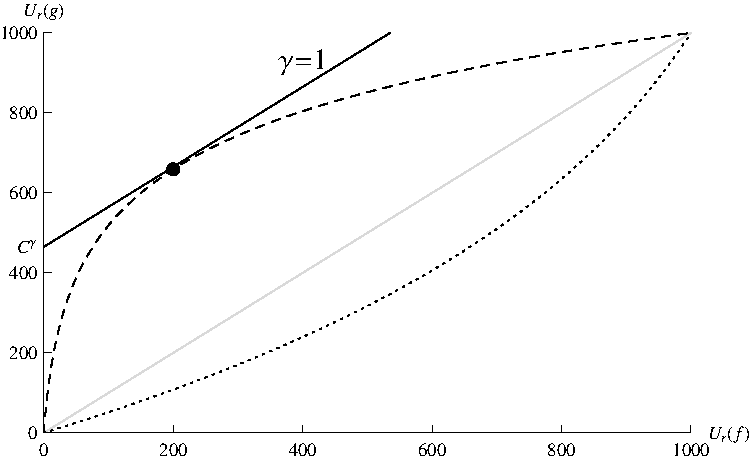
\includegraphics[width=4in]{tangent} }
 \end{figure}

 
 Now consider the general case of the test of $H_j$.  Assume that the alpha
 wealth available to the two investing rules is $A_j$ and $B_j$, respectively,
 at this stage, and that it has been $\ell \le j$ tests since the last rejection
 by the first rule and $m \le j$ tests since the last rejection by the second.
  Assume also for ease of presentation that the level $\al_j = A_j f(\ell)$
 invested in the test of $H_j$ by the first investing rule is less than the
 level $\beta_j = B_j g(m)$ invested by the second ($\al_j < \beta_j$). It
 follows that, when utility is measured by the number of rejections, that we
only need a one-dimensional optimization at each test,
 \begin{eqnarray}
   C^\gamma_j(A_j,\ell;B_j,m) 
    &=& \max_{\mu \in \R } \left[ r^{}_{\mu}(\al_j) - \gamma \, r_{\mu}(\beta_j)\right. \cr
    && \;+ \quad r_{\mu}(\al_j) \qquad \quad
              C^\gamma_{j+1}(A_j+\omega-\alpha_j,0;\,B_j+\omega-\beta_j,0)  \cr
    && \;+ (r_\mu(\beta_j)-r_\mu(\al_j)) \; 
              C_{j+1}^\gamma(A_j-\alpha_j,\ell+1;\,B_j+\omega-\beta_j,0) \cr
    && \;+ \left.  (1-r_\mu(\beta_j)) \; 
              C_{j+1}^\gamma(A_j-\alpha_j,\ell+1;\,B_j-\beta_j,m+1) \right] \;,
 \label{eq:util}
 \end{eqnarray}
 with the boundary condition $C_{T+1}^\gamma = 0$.  The successive lines
 identify the expected differential in the number of rejections produced by the
 test of $H_j$, and following summands denote the subsequent expected values if
 both reject, if only the rule with the larger alpha level rejects, and if
 neither rejects.  


 Practical solution of the recursion for $C_1^\gamma$ requires a discrete
 approximation.  Notice in \eqn{eq:util} that the state of the recursion depends
 on the wealths of the two investing rules. Feasible calculation requires that
 we restrict the possible wealths to a discrete grid.  If the wealths are
 allowed to vary over any $W \ge 0$, then solving this recursion for any sizable
 $T$ is intractable.  Our approach discretizes the wealth functions so that the
 optimization occurs over a grid for each test $j$ rather than the positive
 quadrant of $\R^2$.  For each investing rule, we initialize a grid of $T+M+1$
 wealth values $w_j$, indexed from $j=M, M-1, \ldots, 1, 0, -1, \ldots, -T+1,
 -T$.  This grid holds the state of the wealth at each test, and the differences
 in adjacent wealths determine the amounts used to test the next hypothesis.
  For the rule defined by the distribution $f \in {\cal F}$, we set $w_0 = W_1$,
 $w_{-1} = w_0(1-f(0))$, $w_{-2} = w_{-1}(1-f(1)), \ldots$.  If the investing
 rule does not reject any hypotheses, these wealths are exact.  If the rule does
 reject, we accumulate the utility as though performing a randomized test that
 tosses a biased coin to decide which of the nearby wealths to spend.  Suppose
 that the alpha wealth when rejecting is $X = w_j + \omega$.  It is unlikely
 that $X$ lies at one of the grid of wealth values, so assume that $x = c \, w_k
 + (1-c) w_{k+1}$ for some $0 < c < 1$.  In this case, we treat the next test as
 a randomized test.  The test earns the expected utility from wealth $w_k$ with
 probability $(1-c)$ and from wealth $w_{k+1}$ with probability $c$. Basically,
 this approximation adds a second expectation to the sum in \eqn{eq:util}. We
 set $w_j$ for $j > 0$ somewhat arbitrarily in a manner that prevents the
 accumulation of excess wealth.  In our examples, $M=5$ with $w_i = W_1 + i
 \,\omega/3$, $i=1,2,3$, and $w_i = w_{i-1} + \omega$ for $i=4,\,5$.  Should the
 wealth reach $w_4$, then the bid for the next test is $\omega$, the amount
 earned by a rejection.  Hence, the testing does not increment the wealth beyond
 this boundary.
 

 We obtain a performance envelope by varying the competitive factor $\gamma$.
  To find the boundary points below the diagonal, we reverse the roles of the
 alpha investing rules and repeat the optimization.  As the optimization
 proceeds, we accumulate the component utilities that identify the boundary
 point.


%--------------------------------------------------------------------------
\section{ Examples }
%--------------------------------------------------------------------------
 
 The examples in this section compute the feasible risks produced by the alpha
 investing rules just described.  We also consider several choice for the payoff
 $\omega$ that controls mFDR.  The choices span from the conventional Type I
 error rate with $\omega=0.05$ to $\omega = 0.5$ and larger.  Setting
 $\omega=0.5$ implies that we allow up to half of the rejected hypotheses to be
 Type I errors.  Such a large error rate would not be used in testing, but is
 natural when trying to minimize worst case risk.  

 \clearpage

 A simple approximation suggests that alpha investing procedures should allow
 larger values for mFDR than typical in testing.  Consider the risk produced by
 a testimator defined by a test of simple hypotheses for a mean.  Suppose that a
 test of the hypotheses $H_0: \mu=0$ versus $H_a: \mu=\eta$ has level $\alpha$.
  The test rejects $H_0$ if $Y^2 > z_{\al/2}^2$ for $Y \sim
 N(\mu,1)$.  Our approximations decompose the risk of the testimator
 $\hat\mu_\al = Y\,\one{Y^2>z_{\al/2}^2}$ as shown in the following table. Note that we treat $\mu$ as a
 r.v. with probability $\pi$ on $\eta$ and 0 otherwise.

\begin{center}
\begin{tabular}{c|cc}
            &   $\hat\mu=0$            & $\hat\mu\ne 0$               \cr \hline
 $\mu=0$    &  0                       & $\al (1-\pi) (2 \log 1/\al)$ \cr
 $\mu=\eta$ &  $(\pi/2)(2 \log 1/\al)$ & $\pi/2 \cdot 1$              \cr
\end{tabular}
\end{center}

 \noindent
 These approximations use $z_\al \approx \sqrt{2 \log 1/\al}$ and estimate the
 risk at this threshold by $2 \log \al$.  The components in this table are
 summands in the decomposition
 \begin{equation}
   \ev (\hat\mu_\al - \mu)^2 
     = \sum_{C} \ev \left((\hat\mu_\al-\mu)^2 | C\right) \pr(C),
 \label{eq:decomp}
 \end{equation}
 where the conditions are $\{\mu=0, Y^2 < z_{\al/2}^2\}, \{\mu=0, Y^2 \ge
 z_{\al/2}^2\},\{\mu=\eta, Y^2 < z_{\al/2}^2\},\,\mbox{ and
 },\{\mu=\eta, Y^2 \ge z_{\al/2}^2\}$.


 Now consider the mFDR for this table:
 \begin{equation}
     mFDR = \frac{\al(1-\pi)}
                 {\al(1-\pi) + \pi/2} \;.
 \label{eq:mfdrtable}
 \end{equation}
 To perform well, the testimator should balance the risk associated with the two
 types of errors, so that \ras{Should this balance refer to {\bf both} of terms
 from the second column or just to the Type I and Type II errors? It would not
 make much difference here, but it does in the more accurate calculations. }
 \begin{equation}
   \al(1-\pi) 2 \log (1/\al) \approx (\pi/2) (2 \log(1/\al) \Rightarrow   
         \pi/2 \approx \al(1-\pi) \;.
 \label{eq:balance}
 \end{equation}
 Plugging this back in \eqn{eq:mfdrtable} gives mFDR$=\half$.

 \clearpage

 To make the problem hard, suppose that the mean
 under the alternative has been chosen to produce maximum risk for the
 testimator,
 \begin{equation}
    \mu_\al = \arg \max_\mu R(\hat\mu,\mu) \approx \mbox{[add this]}
 \label{eq:Malpha}
 \end{equation}
 Figure \ref{fi:risk} shows a plot of the risk with $\alpha=0.05$ and
 $\alpha=0.0005$, a more typical value in, say, model selection.
  \citet{fostergeorge94} show that as $\alpha \rightarrow 0$, $\mu_\al = \sqrt{2
 \log 1/\al} + o(something) \approx z_{\al/2}.$ Assume, as in a Bayesian model,
 $H_a$ holds with small probability $\pi$; in other words, we are in the 'nearly
 black' setting in which most parameters are zero.  The major contributions to
 the risk in this setting come from Type I and Type II errors.  The risk from a
 Type I error is large because the test rejects $H_0$ only if $Y$ is far from
 zero: $\alpha (1-\pi) 2 \log(1/\al).$ The risk from a Type II error is also
 large because of the size of $\mu_\al$; this risk is approximately $(\pi/2) 2
 \log(1/\al)$. (The $\pi/2$ comes from the distribution of $Y$ under $H_a$ being
 located on the rejection boundary.)  Setting mFDR equal to 1/2 balances these
two risks.  In this context,
 \begin{equation}
    mFDR = \frac{\al(1-\pi)}
                {\al(1-\pi) + \pi/2} \;.   
 \label{eq:mfdrexample}
 \end{equation}
 Balancing the risks of Type I and Type II errors implies that we set
$\pi/2=\al(1-\pi)$ and hence that we want $mFDR = 1/2$.


\clearpage

 To evaluate an alpha investing rule, we consider its performance in the
 following context.  Consider testing a sequence of $T$ null
 hypotheses $H_j: \mu_j \le 0, \, j=1,\,2,\, \ldots, \mu_T$ versus the alternatives
 $H_{j,a}: \mu_j > 0$.  \marginpar{$\mu_{1:T}$} Denote the collection of mean
 parameters $\mu_{1:T} = \{\mu_1, \mu_2, \ldots, \mu_T\}$.  The test statistics
 are $Z_j \sim N(\mu_j,1)$.  The $Z_j$ are independent and observed one at a
 time; the test of $H_k$ is made in the knowledge of prior $Z_j$ for $j<k$, but
 future $Z_j, j > k$ are unknown.  The number of tests $T$ is fixed and known at
 the start of testing.  For the purpose of calculating risks, a sequence of
 tests defines a sequence of `testimators' by setting $\hat\mu_j = Z_j$ if
 $p_j<\al_j$ and zero otherwise.
 

 

 Within this context, how does the choice of an investing rule influence the
 performance of alpha investing?  Let $U$ denote a figure of merit, or utility,
 provided by using an alpha investing rule.  For example, the utility might be
 the expected number of hypothesis $H_j:\mu_j=0$ rejected by the alpha investing
 rule defined by the distribution $f \in {\cal F}$:
 \begin{eqnarray}
    U_r(\mu_{1:T},\,f) 
      &=& \ev_{\mu_{1:T}} \sum_{j=1}^T r_{\mu_j}(\alpha_j) \label{eq:Ur} \\
      &=& r_{\mu_1}(\al_1) \left( 1 + r_{\mu_2}(W_1-\al_1+\omega) + \cdots \right)\cr
      & &  + (1-r_{\mu_1}(\al_1))\left( r_{\mu_2}(W_1-\al_1) + \cdots \right) \;,
 \label{eq:Ure}
 \end{eqnarray}
 where $r_\mu(\al) = \Phi(\mu - z_\alpha)$ is the probability of rejecting,
 $z_\al = \Phi^{-1}(1-\al)$ is the normal quantile, and $\Phi$ is the cumulative
 standard normal distribution.  In \eqn{eq:Ur}, $\al_j$ denotes the amount
 invested in the test of $H_j$ by following the investing rule defined by the
 distribution $f$; this notation suppresses the detail of how prior rejections
 influence this random variable as suggested by \eqn{eq:Ure} that shows how
 $\al_2$ depends on the prior outcome.  Alternatively, we also measure the
 utility in the sense of accumulated (negative) risk.  If $Z \sim N(\mu,1)$,
 then the risk of the testimator $\hat\mu = Z \,I_{\{Z < z_\al\}}$ is
 \begin{equation}
   R_{\mu}(\al) = (1-r_\mu(\al))\mu^2 + (z_\al-\mu)\phi(z_\al-\mu) + \Phi(\mu-z_\al)
 \label{eq:Rmu}
 \end{equation}
 The associated cumulative utility is then
 \begin{equation}
    U_R(\mu_{1:T},\,f) = \ev_{\mu_{1:T}} \sum_{j=1}^T R_{\mu_j}(\alpha_j) 
 \label{eq:UR}
 \end{equation}
 

 To compare two alpha investing rules defined by $f,\,g \in {\cal F}$, define
 the {\em performance envelope} of $(f,\,g)$ to be the region
 \begin{equation}
    \mbox{PE}(f,g;\rho) = \{(x,\,y) \in \R^2: \exists \; \mu_{1:T} \in \RT \; s.t. \; 
                     x = U_\rho(\mu_{1:T},f),\,  y=U_\rho(\mu_{1:T},g))\} \;.
 \label{eq:PE}
 \end{equation}
 The point $(x,\,y)$ lies in the performance envelope if there exists a sequence
 of means for which these coordinates identify the utilities obtained by the two
 alpha investing rules.  As an example, Figure \eqn{fi:pe} shows PE$(g_{0.11},u;\;
 r)$, the rejection performance envelope of alpha investing with a geometric
 distribution having $\psi = 0.11$ versus the universal distribution $u$ defined
 in \eqn{eq:univ}.  Points within the performance envelope of $(g_{0.11},u)$ that lie
 below the diagonal indicate parameters $\mu_{1:T}$ for which $g_{0.11}$ produces
 higher utility than $u$; those above the diagonal (the larger portion of Figure
 \eqn{fi:pe}) indicate $u$ dominates $g_{0.11}$. In this example, the universal
 distribution dominates the geometric almost everywhere.  The advantage is
 particularly stark near the origin; in this `nearly black' situation, few
 hypotheses are rejected and the universal rule produces far better performance.


 \begin{figure}
 \caption{ \label{fi:pe} Performance envelope PE$(g_{0.11},u;\;r)$ shows the
 expected number of rejected hypotheses obtained by the geometric alpha
 investing rule $g_{0.11}$ versus the universal investing rule ($T=250$)}
 \centerline{ 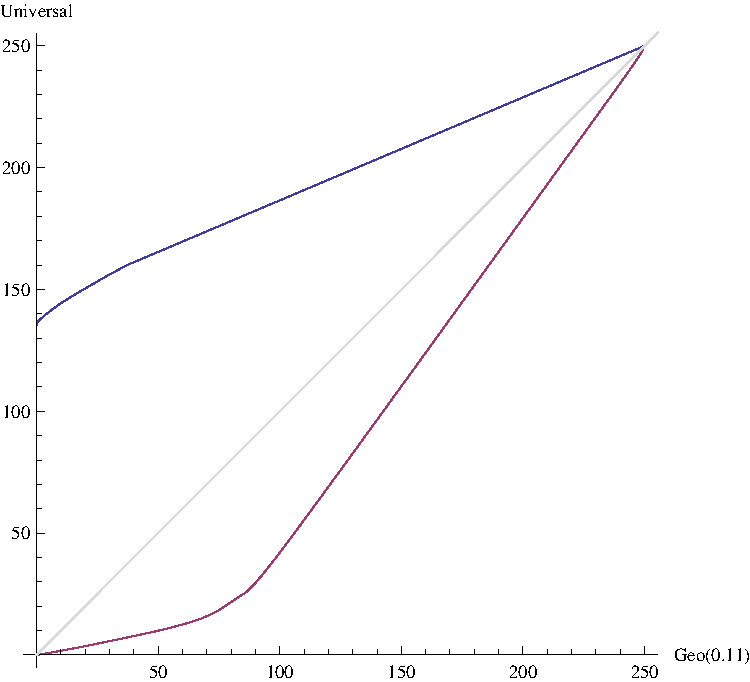
\includegraphics[width=4in]{envelope} }
 \end{figure}


 {\ras Connection to risk inflation.}

 The risk inflation of the testimator
 $\hat\mu_{\hat\gamma}$ is the maximum over choices of $\mu$ (and hence of
 $\gamma$) of the ratio of the risk of $\hat\mu_{\hat\gamma}$ to the smallest
 risk attainable by any testimator:
 \begin{equation}
    \mbox{RI}(\hat\gamma) 
          = \sup_\mu  \frac{R(\mu, \hat\mu_{\hat\gamma})}
                           {\inf_\eta{R(\mu, \hat\mu_\eta)}}   \;,
 \label{eq:ri}
 \end{equation}
 where $\eta \in \{0,1\}^p$ denotes an arbitrary selector.  This version of risk
 inflation is denoted $\widetilde{\mbox{RI}}$ in \citet{fostergeorge94}; the
 more common form restricts the denominator in \eqn{eq:ri} to the risk of the
 ``correct'' testimator, $R(\mu, \hat\mu_\gamma)$.  In that case, the
 denominator reduces to the number of non-zero means, $\sum \gamma_j$.  Foster
 and George show that the properties of these two definitions of risk inflation
 are similar; the version in \eqn{eq:ri} is more natural for our application.
  Given independent simultaneous (rather than sequential) tests,
 RI$(\hat\gamma)$ is asymptotically equal to $2 \log p$.  \citet{fostergeorge94}
 show that
 \begin{equation}
     2 \log p + o(\log p) \le  RI(\hat\gamma) \;,
 \label{eq:lower}
 \end{equation}
 and that hard thresholding (basically, Bonferroni selection) is essentially optimal,
 \begin{equation}
       RI(\gamma_{2 \log p}) < 1 + 2 \log p \;.
 \label{eq:upper}
 \end{equation}
 Comparable results were obtained by \citet{donohojohnstone94} around the same time. 



%--------------------------------------------------------------------------
\section{ Discussion }
%--------------------------------------------------------------------------


 Return to model selection.

  Suppose one has a collection of $p$ variables $X_1, \ldots, X_p$ to consider as
 explanatory variables in the classical linear regression model
 \begin{equation}
   Y_i = \beta_0 + \beta_1 X_{i1} + \cdots + \beta_p X_{ip} + \ep_i, 
     \qquad \ev \ep_i = 0, \Var(\ep_i)=\sigma^2,  \quad i = 1,\ldots,n\;.
 \label{eq:regr}
 \end{equation}
 As a method for picking a model, subset selection (sometimes called $L_0$
 selection) in effect tests the hypotheses $H_j: \beta_j = 0, \; j = 0, 1, \ldots, p$.
  Let $\gamma_j = \pm 1$ denote those $\beta_j \ne 0$, and let $\hat\gamma_j =
 \pm 1$ identify the rejected hypotheses.  The explanatory variable $X_j$
 appears in the fitted model if $\hat\gamma_j = 1$ and is excluded otherwise
 (hence estimating $\beta_j$ = 0).  We insert an intercept in all models (as
 needed by risk inflation below) and so set $\gamma_0=\hat\gamma_0 = 1$.  The
 vectors $\gamma = (1, \gamma_1, \ldots, \gamma_p)'$ and $\hat\gamma = (1,
 \hat\gamma_1, \ldots, \hat\gamma_p)'$ collect these indicators.


Alpha investing can mimic regular testing procedure by revisiting the test of
prior hypotheses. 

Improve the estimator by shrinkage.



One might also use accumulated alpha wealth as a measure of the performance, and
 this provides a more useful metric of performance, particularly when competing
 against the oracle.  If maximizing alpha wealth, then the oracle loses the
 amount bid and chooses $\mu_j$ to maximize $r_{\mu_j}(\al)-\al$ rather than
 $r_{\mu_j}(\al)$ alone.  This perspective would not only capture aspects of
 rejecting hypotheses, it also anticipates having resources to test future
 hypotheses.  Such consideration is appropriate, however, only in the context of
 testing a larger collection of hypotheses than considered here.

 \ras{ Things left to do:
 \begin{enumerate}
 \item Graphs of envelope that suggest that alpha wealth is a decent proxy for
 risk, at least better than something like FDR, number rejects - constant times
 number false rejects.
 \item What does the steady state look like.  If take the envelope for 250 and
 double to get for 500, is that close to correct for the risk?
 \item Comment on the value of saving if hope to compete with a universal
 bidder.
\end{enumerate}
}


%--------------------------------------------------------------------------
\section{ Bibliography }
\section*{Acknowledgement}
%--------------------------------------------------------------------------

The authors thank ...


%--------------------------------------------------------------------------
% References
%--------------------------------------------------------------------------

\bibliography{../../../../references/stat}
\bibliographystyle{../../bst/asa}

\end{document} %==========================================================
